\chapter{Prior and related work}
My research rests on the previous contribution by many people to three research areas: 
software repository mining, time-series analysis, and information retrieval. By adopting and combining existing
techniques from these areas I have developed a generic workflow and implemented a software toolkit, 
that enables researchers and practitioners to discover significant recurrent behaviors.

\section{Software process discovery}
Engineers build things and make them work by applying known theories, methods, 
and tools, appropriately and selectively, in systematic fashion, to reach the goal. 
It is also widely recognized, that the process of engineering is conducted 
within an \textit{externally restricted} environment - engineers comply with organizational rules, 
financial restrictions, and schedule. Altogether - these methods and principles 
control the process of engineering, assuring it safety for life and property, 
and making engineering result predictable. 
Inspired by aforementioned structured approach, as mentioned before,
the independent discipline originally called computer programming was 
brought under an umbrella of the software engineering in order to tame an increasing 
complexity of software design processes.




The new engineering discipline - Software Engineering (SE) was born in 1968, 
when the first NATO Software Engineering Conference was held. It is thought, 
that the assignment of computer programming into an engineering discipline 
was made with intent to bring that somewhat unpredictable and disorganized 
activities into the streamlined and controlled environment. 
Thus, similarly to many other engineering disciplines, Software Engineering was 
defined as the application of a systematic, disciplined, quantifiable 
approach to the design, development, operation, and maintenance of the 
final product - the software.
Delivering high quality software products within the budget and in 
time was set as the main goal and the most challenging task 
of Software Engineering.

As said before, back then, the Software Engineering thought to be not different 
from other engineering fields. Using existing engineering tradition, researchers 
and practitioners designed a number software development processes providing 
detailed guidelines on how to reach the goal efficiently and in time. 
These processes manifested themselves as the means for improvements in terms of quality, 
speed, and execution cost over existing practices. They were studied within academic 
settings and adopted by industry. Some of this processes were further standardized, 
shaping the best practices of contemporary 
software development \cite{citeulike:9962021}. 

The processes, that I am addressing here, found in numerous studies and described at length in 
academic and industrial literature. Too numerous to name, they can be categorized by the level 
of their application:
\begin{itemize}
 \item global organizational standards, like CMMI, ISO 9000, and SPICE. 
 \item large industrial software models, such as Waterfall, Spiral, Cleanroom, etc.
 \item smaller scale, flexible methodologies and agile approaches: XP, SCRUM, FDD, 
TDD, Pair Programming, etc.
 \item general guidelines and principles aiming to improve the software process flow, 
such as ``build before commit'' and others.
 \item and finally, there are processes for improving existing processes of software development 
on the organizational, team, and personal levels: TSP, PSP, Six Sigma, etc.
\end{itemize}
While some of these are products of a ``technology transfer'' - resulted by direct copying or by an 
application of existing engineering principles to software development process (like Waterfall model), 
some, and in particular agile methods, considered to be a software-engineering only processes. 

\subsection{Mining software repositories}

\section{Knowledge discovery in time series}

\section{Recurrent behaviors discovery from software process artifacts}

\section{Motivation}
Engineers build things and make them work by applying known theories, methods, 
and tools, appropriately and selectively, in systematic fashion, to reach the goal. 
It is also widely recognized, that the process of engineering is conducted 
within a restricted environment - engineers comply with organizational rules, 
financial restrictions, and schedule. Altogether - these methods and principles 
control the process of engineering, assuring it safety for life and property, 
and making engineering result predictable. Currently, engineering is considered to 
consist of four branches each of which consists of dozens of sub-disciplines. 
There are also numerous interdisciplinary 
engineering fields and many extensions as well. 

The new engineering discipline - Software Engineering (SE) was born in 1968, 
when the first NATO Software Engineering Conference was held. It is thought, 
that the assignment of computer programming into an engineering discipline 
was made with intent to bring that somewhat unpredictable and disorganized 
activities into the streamlined and controlled environment. 
Thus, similarly to many other engineering disciplines, Software Engineering was 
defined as the application of a systematic, disciplined, quantifiable 
approach to the design, development, operation, and maintenance of the 
final product - the software.
Delivering high quality software products within the budget and in 
time was set as the main goal and the most challenging task 
of Software Engineering.

As said before, back then, the Software Engineering thought to be not different 
from other engineering fields. Using existing engineering tradition, researchers 
and practitioners designed a number software development processes providing 
detailed guidelines on how to reach the goal efficiently and in time. 
These processes manifested themselves as the means for improvements in terms of quality, 
speed, and execution cost over existing practices. They were studied within academic 
settings and adopted by industry. Some of this processes were further standardized, 
shaping the best practices of contemporary 
software development \cite{citeulike:9962021}. 

The processes, that I am addressing here, found in numerous studies and described at length in 
academic and industrial literature. Too numerous to name, they can be categorized by the level 
of their application:
\begin{itemize}
 \item global organizational standards, like CMMI, ISO 9000, and SPICE. 
 \item large industrial software models, such as Waterfall, Spiral, Cleanroom, etc.
 \item smaller scale, flexible methodologies and agile approaches: XP, SCRUM, FDD, 
TDD, Pair Programming, etc.
 \item general guidelines and principles aiming to improve the software process flow, 
such as ``build before commit'' and others.
 \item and finally, there are processes for improving existing processes of software development 
on the organizational, team, and personal levels: TSP, PSP, Six Sigma, etc.
\end{itemize}
While some of these are products of a ``technology transfer'' - resulted by direct copying or by an 
application of existing engineering principles to software development process (like Waterfall model), 
some, and in particular agile methods, considered to be a software-engineering only processes. 

\section{Motivation}
As shown before, there are numerous software process, models, methodologies, and 
coding conventions exist for any level and any stage of the software development 
processes carried out by any arbitrary team size at any scale. 
This amount of well-grounded and documented knowledge creates an impression, 
that the area of software development process is thoroughly explored, 
and that there exists a deterministic choice for a model and a 
processes for any software project. 
In other words, the amount of our knowledge about how to engineer the software, 
leaves no doubts in the the faith of softare projects - that they will be completed 
succesfully. 

However, it is far from being true - software projects still fail at the considerably 
high rate and many unforeseen challenges exist in software product development.
This phenomena, also known as a ``software crisis'', was first recognized by Randell et al. in 1976 
\cite{naur1976software}. The attention was caught by the fact that many software projects ran 
over budget and schedule, some caused property damage \cite{citeulike:11044022}, and a few projects caused 
loss of life \cite{citeulike:712058}. Decades later, the ``Chaos Report'' from the Standish 
Group \cite{SDTimes} state, that only ``35\% of software projects in 2006 can 
be categorized as successful - meaning they were completed on time, on budget and met 
user requirements''. These thirty five percent of success clearly manifest that it is somewhat 
illusory statement that we are capable to understand and to control software processes.

This rather poor performance of the mainstream software engineering processes 
ignited a new wave of research in the field in recent decades. Gradually, researchers and 
practitioners alike recognized, that a direct application of classical engineering and a 
straightforward ``up-down'' software process governing might be somewhat erroneous. 
Also, it was recognized that over many years, continuous formalization of the field and 
excessive attention to software process metrics may malformed not only the software development 
practices landscape, but education and a professional code of conduct. 
This recognition forced some of the professional associations 
to review their licensing policies \cite{citeulike:11045517} and some educators to change their 
opinions \cite{citeulike:5203446}. 

In parallel with this search for industrial ``software crisis'' solution, another phenomena, 
the Open Source Software (OSS) 
development - an alternative software process arose and has proven its ability to deliver 
large, high quality software products. The OSS process is largely differ from typical SE process
on many levels - first of all it is carried out by a highly distributed community of people,
which significantly contradicts to developers collocation assumed by the most of the SE processes.
Secondly - OSS delivers a software free of charge and promotes its reuse, modification, and 
redistribution by anyone, moreover the OSS software is largely developed for a fraction of cost
of similar commercial projects. And finally, the OSS projects rarely governed by or can provide
any sort of documented software process. Yet, many OSS projects delivered large-scale, widely
adopted software systems fully comparable or superior to industrial projects.

Lately, third approach to software development emerged - software craftsmanship emerged 
\cite{citeulike:11058561}, \cite{citeulike:11058554}. The followers of this methodology 
are not only focused on the delivering ``well crafted'' software and continuously adding value,
but on the apprenticeship - on forming communities and engaging more people in software development.
While recommendation exists \cite{citeulike:11058784}, little known about the research 
in software craftsmanship and apprenticeship processes.

All this continues to engage thoughts and fuels the search not just for the exact definition 
of software development, but deep, fundamental for efficient processes resolving. 
Is software development an engineering discipline? Is it a craft \cite{citeulike:5203446}? 
Or is it an art \cite{citeulike:11045694}?

Answers to these questions would require extensive interdisciplinary studies to be made, 
but what is obviously clear, is that formal software development process, as an engineering 
is a creative, human activity. 
Whether software is coded 
by team where its members have a variety of skills and experience, or by a single individual,
they all driven by their believes and motivations. While usually developers agree on the use of 
particular technologies, development tools, and a development process with imposed timeline and 
a budget, the software process is - as many other human activities - highly creative and mostly 
non-recurring. Thus, the choice of methodology, technology, or tools provides only a marginal 
effect on this human-based and human-driven process. While this effect can be measured through 
the common approach by using a control environment factoring out human component, the most of 
the difference, which lies in human creativity, motivation and productivity is unknown and yet, 
mostly immeasurable.

\section{Research area overview}
\todo[inline]{here, describe in short the current state of the art and notable efforts which
shed light on the research area and identify a precise place where I am going.}
Here, lies a great room for the research and for improvement of our understanding of software 
processes. And my thesis is yet another attempt at the understanding of the role human activities 
in the software process. Before going further, I would like to emphasize, that in this work I will not 
address the need and means of the process synthesis, process quality assessment, productiveness
or any topics related to the software product itself; I would rather focus on the specific issue - 
on uncovering an existence and on studying the programming habits. 

\chapter{Background work}
This chapter presents an overview of my research background and a targeted literature 
review of previous work, closely related to the research problem.
The relevant theory is examined for each domain: software engineering and software process
in particular, process mining, activity (behaviors) patterns theory and analysis, and 
a timeseries analysis. Each section provides a concise review of related work, discussion 
of constructs and a summary explaining their relevance and applicability. 

Section \ref{software.processes} includes the general principles and properties of 
software process models, as well as a discussion of the current research in the area.
Section \ref{oss.processes} reviews studies in Open-Source software processes
explaining foundations for OSS processes and their recovery.
Section \ref{activity} includes a discussion of the activities performed within software
process, their meaning, and their relation to recurrent behaviors.

\section{Terminology}\label{definitions}
The number of terms and expressions is used throughout this thesis. This chapter provides
their definitions and detailed explanations.

\textit{\textbf{Artifact}} in software engineering, is a generic term used for identification
of many kinds of software process byproducts such as specification documents, use cases, 
risk assesments, defect reports, etc. These are called byproducts because this entities
arise from the performing process itself rather than being the results produced by the process.

The subset of software process artifacts, which is particularly relevant for my thesis, 
and will be examined and used thorougly, is the set of software change artifacts - 
elctronic records which stem out of the software change processes.

\textit{\textbf{Process}} in engineering, is a term usually used for a set of interrelated 
steps which transform an input into desired output. These steps are carried out by the process
enactors: people, machines, or natural forces. 

In software engineering, the meaning of process is similar to that and used for a set of steps 
which are designed to transform some input software artifacts (the code, design documents, 
or use cases) into desired output, which can be a transformed version of input, or a
distinct product. For example, code review process is designed to transform an input - the 
source code into an output - a list of defects.

However, in this thesis, I will use perm \textit{\textbf{process}} as an umbrella term for 
larger sets of software-engineering entities which meant to impose a structure or order on
the software development activity. These entities include, but not limited to a software 
development life cycle model, software method or techniques, rules or action plans. 

\textit{\textbf{Methodology}}, according to the Oxford dictionary, is defined as a system of 
methods used in a particular area of study or activity. In context of this thesis the 
term methodology is used for a guideline system aiming on solving a problem. Usually, 
methodology consist of specific components such as tasks, methods, techniques and tools, 
and usually applied in phases. Overall methodology is not a single method, but rather 
a processes to be followed, a generic framework that can be further broken down into 
sub-processes.

\textit{\textbf{Method}}, according to the Oxford dictionary, is a particular procedure for 
accomplishing or approaching something, especially a systematic or established one.

\textit{\textbf{Behavior}} in context of this thesis is the range of actions performed by 
individuals or a team in a response to internal or external stimuli. These stimuli can be
further classified on conscious or subconscious, and voluntary or involuntary. 

The terms process and behavior are interconnected in the context of software development
in a sense that human behaviors in software development activity thought to be largely influenced 
by software processes. Nevertheless, whether modulated by software process, or just 
performed arbitrary, activities performed within software development cycle will be called 
behaviors in the context of this thesis.

\textit{\textbf{Temporal structure}} in context of this thesis is the temporal pattern of
a single activity or a set of activities performed by individual or a group. 

\textit{\textbf{Activity cycle}}, or \textit{\textbf{temporal container}} in context of 
this thesis is an abstraction of temporal window containing temporal structure (structures).

\section{Software processes}\label{software.processes}
There are different approaches for software development which were designed in order to 
facilitate the creation of software systems. These approaches provide means for 
structuring of development activity. The main goal of imposing such a structure on the 
development process is to organize production of code in manageable way. 
According to the research, structuring software process yields a number of benefits:
\begin{itemize}
 \item whole software development cycle can be broken down onto number of one-step pieces;
 \item which, in turn, helps to keep clear focus on what must be delivered and when, during each step;
 \item it clarifies the project scope and improves time, effort, and cost estimates;
 \item it provides ability to measure the progress;
\end{itemize}
It is strongly advocated, that the use of established and well structured process is 
essential for the complex projects in order to orchestrate collaborative effort 
of multiple teams. 

\subsection{Software process models}
Structuring software development includes the use of a software process model and following 
a software method, known as methodology. While latter is used primarily to navigate 
through the development process: determining a number of functional points, 
designing data flow diagrams, etc., the model provides developers with guidance about their 
tasks and the software development activities that should be undertaken. 
This definition of steps and ordering of carried activities facilitates
a framework for estimation of resources, defines major milestones, and provides 
means for time and effort monitoring and management. 

All of software process models include three generic steps, or high-level phases, 
corresponding to software life cycle: definition phase, development phase, and a maintenance phase. 
The definition phase includes the initial planning of the future system and 
the requirements collection: developers identify data need to be processed by the system, 
its functionality, behavior, and what constraints must be placed on the system design 
and development. 
The development phase focuses on the system implementation and testing: 
developers write the system code, test if the system satisfies to user requirements, 
has planned behavior, and produces needed output. 
The last, maintenance phase, focuses on the post-development activities: 
system deployment and its operational support. 

In each software model these large phases are composed of series of smaller, distinct phases.
Each of these phases is executed with a particular 
goal: some will provide a part of the software system, or perform its validation, 
while other will deliver the engineering documentation, or a user manual. 
Examples of such phases are the requirements collection, user manual writing, 
coding of a a functional module, etc.
The determination of these small phases, its ordering, and the definition of the phase-transitioning 
criteria are different from model to model.

\todo[inline]{should I put examples of models to here, their key advantages and disadvantages?}

\subsection{Software process modeling research}
The research area dealing with Software Process Modeling (SPM) was receiving significant 
attention over the years and is recognized as one of the powerful technologies
in software process engineering. The empirical approach techniques play a critical role
in SPM and most of the work is based on the case studies and action research. 
However, this approach has an intrinsic flaw - it is hardly feasible since
empirical SPM research activities are limited by organizational context, and also extremely 
expensive - some of the known reports required decades to obtain an empirical evidence.
Thus, in most cases, it is unfeasible to perform an explanatory research in full rigor,
and as pointed in \cite{citeulike:11079867}: ``Currently the empirical studies in SPM were 
mostly exploratory in nature, whose strengths of empirical evidence were relatively weak...''
\todo[inline]{process modeling built up-down and it is expensive!}

\subsection{Software process elicitation and conformance}
Another area of research related to my work is the area of the software process conformance. 
the research in this area is dealing with methods and theories for formulating, identifying and
investigating violations in the execution of software processes. These methods heavily rely
on the process elicitation step which is of most interest \todo[inline]{very similar}. 

\todo[inline]{Paragraph about ``classical'' software process research - heavyweight, expensive
mostly top-down oriented: first designed, secondly tested or confirmed}.

\section{Open Source Software processes}\label{oss.processes}
In recent time we have seen the rise of alternative software development practices. 
With development of communication technologies, groups of people were 
enabled to collaborate together over the Internet in order to create software that is 
licensed openly promoting software reuse, modification, and distribution. While there are 
hundreds of thousands of open source projects, they rarely provide any explicit details on 
their software processes, moreover, they often refuse to provide any of 
specifications \cite{Torvalds:2005}. 

From little which is known about OSS processes, they are quite different from what is 
commonly thought in the classrooms or what industrial standards tell us.

\subsection{Death of distance and cyberspace}
With the development of internet infrastructure connecting continents with ``information
superhighways'', the term ``cyberspace'', once a buzzword \cite{citeulike:11095763}, become 
a term which explicitly refer to the real-world phenomena providing an information-exchange
and collaborative medium. Unlike traditional physical space and transportation networks, where 
materials and workers are transported at limited speeds in space and time, the information 
superhighways in cyberspace form networks for digital information to be transported almost instantly 
between sites any time and at almost any place. 
Novel communication and collaboration techniques such as videoconferencing and software change 
control systems offer developers great flexibility to control their interaction and collaboration. 
It is possible to interact synchronously or asynchronously from any location and at any time. 
Once software project and developers are online, in cyberspace, not only geographic measures, but 
any geographic notions that are based on the principle of distance friction, such as distance decay,
are not longer applicable to participants and to the software product.

\subsection{Relaxation of space-time constraints, extensibility and displacement}
Time and space constraints significantly influence and shape human activities. There are 
particular research areas dedicated to study the effect of these constraints on individuals 
and society. For example the Hägerstrand's time geography in the Regional science and is 
a powerful conceptual framework which integrates the temporal and spatial dimensions of
human activity patterns. It conceives and represents an individual’s activities and travel 
in a 24-hour day as a continuous temporal sequence in geographical space. The trajectory 
traces this activity sequence as a space-time path in a 3D space-time container composed by a
geographic plane and a Z-axis representing a time dimension. Using this framework, researchers
build space-time paths, illustrating how a person navigates through a spatial-temporal environment.
Using this framework, Hägerstrand demonstrated that human spatial activities are often governed by
three types of constraints: capability, coupling, and authority. Here, the capability constraints
refer to the limitations on human movements due to physical or biological factors, for
example, a person cannot be in two places at one time, but not anymore - however cyberspace allows 
one to actually be present in two places virtually - two chat rooms, or video-conferences.
A coupling constraint refers to the need to be in one particular place for a given length of time 
to be in interaction with other people, not anymore again, high frequency asynchronous
information exchange allows one not only to be ``coupled'' to multiple people, but to multiple 
people in multiple places. And the third constraints, an authority constraint refers to an 
area that is not accessible to particular individuals or groups, which is also shrinked.
\todo[inline]{nice explanation of how cyberspace and OSS relaxed all three}

Basically

\subsection{The Bazaar model and impact of small changes on the process visibility}
\begin{figure}[tbp]
   \centering
   \includegraphics[height=125mm]{commit-often.eps}
   \caption{Illustration of the contemporary trend advocating small commits. 
\url{http://stackoverflow.com/questions/107264/how-often-to-commit-changes-to-source-control}}
   \label{fig:commit-often}
\end{figure}


\subsection{OSS process research}
\subsection{Mining Software Repositories}\label{background.msr.summary}
%\subsection{Mining Software Repositories}\label{mackground.msr.summary}
%%\subsection{Mining Software Repositories}\label{mackground.msr.summary}
%%\subsection{Mining Software Repositories}\label{mackground.msr.summary}
%\input{background_msr_summary}
According to Kagdi et al. \cite{citeulike:4534888} the term \textit{mining
software repositories (MSR)} ``... has been coined to describe a broad class of
investigations into the examination of software repositories.'' The ``software
repositories'' here refer to various sources containing artifacts produced by
software process. Examples of such sources are version-control systems (CVS,
SVN, etc.), requirements/change/bug control systems (Bugzilla, Trac etc.),
mailing lists archives and social networks. These repositories have different
purposes but they support a single goal - a software change which is the single
unit of the software evolution. 

In the literature, \textit{software change} defined as an addition, deletion or
modification of any software artifact such as requirement, design document, test
case, function in the source code, etc. Typically, software change is realized
as the source code modification; and while version control system keeps track of
actual source code changes, other repositories track various artifacts (called
\textit{metadata}) about these changes: a description of a rationale behind a
change, tracking number assigned to a change, assignment to a particular
developer, communications among developers about a change, etc.

Researchers mine this wealth of data from repositories in order to extract
relevant information and discover relationships about a particular evolutionary
characteristic. For example, one may be interested in the growth of a system
during each change, or reuse of components from version to version. Later in this
thesis I will review MSR research field in detail highlighting relevant to my
research work and comparing my results with existing MSR findings.
According to Kagdi et al. \cite{citeulike:4534888} the term \textit{mining
software repositories (MSR)} ``... has been coined to describe a broad class of
investigations into the examination of software repositories.'' The ``software
repositories'' here refer to various sources containing artifacts produced by
software process. Examples of such sources are version-control systems (CVS,
SVN, etc.), requirements/change/bug control systems (Bugzilla, Trac etc.),
mailing lists archives and social networks. These repositories have different
purposes but they support a single goal - a software change which is the single
unit of the software evolution. 

In the literature, \textit{software change} defined as an addition, deletion or
modification of any software artifact such as requirement, design document, test
case, function in the source code, etc. Typically, software change is realized
as the source code modification; and while version control system keeps track of
actual source code changes, other repositories track various artifacts (called
\textit{metadata}) about these changes: a description of a rationale behind a
change, tracking number assigned to a change, assignment to a particular
developer, communications among developers about a change, etc.

Researchers mine this wealth of data from repositories in order to extract
relevant information and discover relationships about a particular evolutionary
characteristic. For example, one may be interested in the growth of a system
during each change, or reuse of components from version to version. Later in this
thesis I will review MSR research field in detail highlighting relevant to my
research work and comparing my results with existing MSR findings.
According to Kagdi et al. \cite{citeulike:4534888} the term \textit{mining
software repositories (MSR)} ``... has been coined to describe a broad class of
investigations into the examination of software repositories.'' The ``software
repositories'' here refer to various sources containing artifacts produced by
software process. Examples of such sources are version-control systems (CVS,
SVN, etc.), requirements/change/bug control systems (Bugzilla, Trac etc.),
mailing lists archives and social networks. These repositories have different
purposes but they support a single goal - a software change which is the single
unit of the software evolution. 

In the literature, \textit{software change} defined as an addition, deletion or
modification of any software artifact such as requirement, design document, test
case, function in the source code, etc. Typically, software change is realized
as the source code modification; and while version control system keeps track of
actual source code changes, other repositories track various artifacts (called
\textit{metadata}) about these changes: a description of a rationale behind a
change, tracking number assigned to a change, assignment to a particular
developer, communications among developers about a change, etc.

Researchers mine this wealth of data from repositories in order to extract
relevant information and discover relationships about a particular evolutionary
characteristic. For example, one may be interested in the growth of a system
during each change, or reuse of components from version to version. Later in this
thesis I will review MSR research field in detail highlighting relevant to my
research work and comparing my results with existing MSR findings.

\section{Evidence of recurrent behaviors}

\section{Activity fragmentation, Activity-based modeling}\label{activity}

\section{Literature search overview}

\section{Process mining}
The recognition of interest and importance of various processes 
According to the IEEE Task Force on Process Mining, established in 2009, ``Process mining is 
a relatively young research discipline that sits between computational intelligence and data 
mining on the one hand, and process modeling and analysis on the other hand'' \cite{citeulike:11077707}.
This group promotes the topic of process mining in three major axes: process discovery,
process conformance checking, and process enhancement 

\subsection{Workflow mining, Business process mining}\label{mackground.bpm}
Although process mining in the business domain is a well-established field with 
much software developed up to date (ERP, WFM and other systems), 
``Business Process Intelligence'' tools usually do not perform process discovery
and typically offer relatively simple analyzes that depend upon a correct
a-priori process model \cite{citeulike:3718014} \cite{citeulike:5044991}.
Moreover, they heavily depend on well composed and annotated process logs as
required by process mining manifesto \cite{citeulike:11077707}:
``All process mining techniques assume that it is possible to sequentially 
record events such that each event refers to an activity (i.e., a well-defined 
step in some process) and is related to a particular case (i.e., a process instance).''

This facts restricts direct application of business domain process mining techniques
to software engineering, where processes are usually performed concurrently by
many agents, are more complex and typically have a higher level of noise. Taking
this fact in account, I will review only the approaches to the mining for which
applicability to software process mining was expressed. 

A set of findings relevant to my research approach was developed by Rubin
et al. \cite{citeulike:1885717} and van der Aalst et al.
\cite{citeulike:3718014} and is called \textit{incremental workflow mining}. The
authors not only designed sophisticated algorithms but built a software system
using a business process mining framework called ProM by van Dongen et al.
\cite{citeulike:5043673} which synthesizes a Petri Net corresponding to the
observed process. The system was tested on SCM logs and while the process
artifacts retrieved from the SCM system are rather high-level, the approach
discussed is very promising for the modeling of software processes from the
low-level product and process data.

\begin{figure}[tbp]
   \centering
   \includegraphics[height=65mm]{petri-log.eps}
   \caption{Illustration of the required log pre-processing step step 
before BPI tools application from \cite{citeulike:1885717}. During this step,
the development log is annotated manually.}
   \label{fig:petri-log}
\end{figure}

\begin{figure}[tbp]
   \centering
   \includegraphics[height=65mm]{petri.eps}
   \caption{Illustration of the ``Generation and Synthesis Approach'' from
\cite{citeulike:5043673}: a) Transition System with regions shown; b),c) Petri
Nets synthesized from the Transition System.}
   \label{fig:petri}
\end{figure}

Within the incremental workflow mining framework, the input data from the SCM
audit trail information is mapped to the event chain which corresponds to the
software process artifacts. The authors call this process \textit{abstraction on
the log level} which is implemented as a set of filters which not only
aggregates basic events into single high-level entities but also removes data
irrelevant to the mining process (noise). 

The event chain constructed through the abstraction is then treated with the
\textit{Generate} part of the \textit{``Generate and Synthesis''}
\cite{citeulike:3718014} algorithm in order to generate a \textit{Transition
System} which represents an ordered series of events. This algorithm looks at
the history (prefix) and the future (suffix) sequences of events related to the
current one in order to discover transitions.  When applied to the abstracted
log information, the algorithm generates a rather large Transition System graph
where edges connect to abstracted events. This transition system is then
successively simplified by using various reduction strategies such as ``Kill
Loops'', ``Extend'', ``Merge by Output'' and others; it is possible to combine
these reduction strategies in order to achieve a greater simplification.

At the last step of the incremental workflow mining approach, Transition Systems
are used to \textit{Synthesize} labeled Petri nets (where different transition
can refer to the same event) with the help of \textit{``regions theory''}
\cite{citeulike:5128170}. As with the Transition System generation, the authors
investigate many different strategies of Petri nets synthesis, showing
significant variability in the results achieved. (see Figure \ref{fig:petri}).

The significant contribution of this research is in the generality of the
method. It was shown that by tuning the ``Generate'' and ``Synthesize'' phases
it is possible to tailor the algorithm to a wide variety of processes. In
particular, as mentioned before, Rubin et al. successfully applied this
framework to the SCM logs analysis.

\subsection{Software process mining and discovery}\label{mackground.bpm}
\section{Mining software repositories}\label{evolution.discovery}
According to Kagdi et al. \cite{citeulike:4534888} the term \textit{mining
software repositories (MSR)} ``... has been coined to describe a broad class of
investigations into the examination of software repositories.'' The ``software
repositories'' here refer to various sources containing artifacts produced by
software process. Examples of such sources are version-control systems (CVS,
SVN, etc.), requirements/change/bug control systems (Bugzilla, Trac etc.),
mailing lists archives and social networks. These repositories have different
purposes but they support a single goal - a software change which is the single
unit of the software evolution. 

In the literature, \textit{software change} defined as an addition, deletion or
modification of any software artifact such as requirement, design document, test
case, function in the source code, etc. Typically, software change is realized
as the source code modification; and while version control system keeps track of
actual source code changes, other repositories track various artifacts (called
\textit{metadata}) about these changes: a description of a rationale behind a
change, tracking number assigned to a change, assignment to a particular
developer, communications among developers about a change, etc.

Researchers mine this wealth of data from repositories in order to extract
relevant information and discover relationships about a particular evolutionary
characteristic. For example, one may be interested in the growth of a system
during each change, or reuse of components from version to version. In this
section I will review some MSR research literature which is relevant to my
research and based on the mining of temporal patterns from SCM audit trails.

\subsection{Mining evolutionary coupling and changes}
One of the approaches in MSR mining relevant to my research is built upon mining
of the simultaneous changes occurring in software evolution. This type of mining
considers changes in the code within a short time-window interval which occur
recurrently. Such changes are revealing logical coupling within the code which
can not be captured by the static code analysis tools. This knowledge allows
researcher and analysts predict the required effort and impact of changes with a
higher precision. 

Mining of evolutionary coupling is typically performed on different levels of
code abstraction: Zimmermann et al. in \cite{citeulike:4406375} discuss mining
of version archives on the level of the lines of source-code using annotation
graphs; Ying et al. in \cite{citeulike:983796} discuss mining of version
archives for \textit{co-change} patterns among files by employing association
rule mining algorithm, and refining results by introducing
\textit{interestingness} measure, which based on the call and usage patterns
along with inheritance; Gall et al. in \cite{citeulike:5397994} use a
window-based heuristics on CVS logs for uncovering logical couplings and change
patterns on the module/package level. Kim et al. in \cite{citeulike:5375867}
taking a different approach by mining \textit{function signature change} and
introducing kinds of signature changes and its metrics in order to understand
and predict future evolution patterns and aid software evolution analysis.

The fine-grain mining of changes on the level of lines of source code is usually
implemented with the use of \textit{diff} utilities family which report
differences between versions of the same file. For capturing temporal properties
the sliding-window approach is used if mining CVS logs, while Subversion is able
to report co-changed filesets (\textit{change-sets}). Use of the information
extracted by parsing issue/bug tracking logs and developer comments from version
control logs allows to capture co-occurring changes with higher precision.

What is common among all this work is that while researchers use different
sources and abstraction levels of information, they are extracting only the
relevant to a specific question data (using filters and taxonomy mappings) and
compose data sets suitable for KDD algorithms. In order to refine and classify
(prune) reported results, various support functions proposed.

The main contribution of this type of mining is in the discovery of patterns in
software changes which are improving our  understanding of the software and
allowing estimation of effort and impact of new changes with higher precision.

\subsection{Ordered change patterns}
A step ahead in the analysis of co-occurring changes in source code entities was
shown by Kagdi et al. in \cite{citeulike:3929070}. The authors investigated a
problem of mining ordered sequences of changed files from change-sets. Six
heuristics (\textit{Day, Author, File, Author-date, Author-file, and Day-file})
based on the version control transaction properties were developed and
implemented. Abstracted sequences were mined with Apriori algorithm (see
\ref{apriori}) discovering recurrent sequential patterns. The authors proposed a
higher specificity and effectiveness of such approach to software change
prediction than by using convenient (un-ordered) change patterns mining.

\subsection{Usage patterns}
Another interesting approach for MSR, relevant to my work, is the mining of
usage patterns proposed by Livshits \& Zimmermann in \cite{citeulike:5398684}.
In this work, the authors approach a problem of finding violations of
application-specific coding rules which are ultimately responsible for a number
of errors. They designed approach to find ``surprise patterns'' (see Subsection
\ref{tpatterns}) of the API and function usage in SCM audit trail by
implementing a preprocessing of the functional calls and mining aggregated data
with a customized Apriori algorithm (see \ref{apriori}) implementation. By
considering past changes and bug fixes, authors were able to classify patterns
into three categories: \textit{valid patterns}, \textit{likely error} patterns,
and \textit{unlikely} patterns. Candidate patterns found with Apriori algorithms
were considered to be a valid pattern if they were found a specified number of
times and an unlikely patterns otherwise. Similarly, if a previously labeled as
valid pattern was later violated a certain number of times, it was considered as
an error pattern. The authors validated their approach on mining publicly
available repositories effectively reporting error patterns.


\section{Temporal data mining}
\subsection{Survey of temporal patterns mining}
\subsection{Symbolic aggregate approximation}

\section{Summary of literature review}

\section{Hypothesized relations between activity patterns and CSDL cycle}

\section{Activity Patterns Frequency and Activity Patterns Entropy as metrics}

\section{Research objectives}